\section{Experimental results and analyses}
Due to the short time and length of Seminar's study, the above does not provide a specific 
analysis of the algorithm's formulas and derivations. We refer to the experimental 
results in the paper by Chen et al.\cite{b15} Their experimental environment is 2.8GHZ Intel Core 
i5,8GB RAM, OS X Yosemite operating system. The algorithm is based on JAVA implementation. 
The algorithm is implemented in JAVA, and the widely used metrics of Mean Absolute Error$MAE$ 
and Root Mean Square Error $RMSE$ are used to measure the performance of the recommender 
system. The dataset is selected for experiments on real datasets, the movie recommendation 
website FilmTrust and the social e-commerce website Epinions.The dataset contains 
information about users' ratings of items and information about trust between users\cite{b24}.

\subsection{Effects of parameters}
Chen et al.\cite{b15} tuned the parameters in their experiments and found that numerous parameters 
affected the recommendation results of the trust algorithm. Here we take the number 
of iterations as an example. At first, the recommendation error decreases as the number 
of training times increases, and then gradually tends to converge\cite{b23, b25}. The number of iterations 
required to minimize the error is different in different datasets. When the number of 
iterations is 80 and 40, the recommendation accuracy of Trust-PMF on FilmTrust and Epinions 
reaches the highest, and the recommendation errors on the two datasets are minimized\cite{b21}.

\begin{figure}[H] %H为当前位置,!htb为忽略美学标准,htbp为浮动图形
    \centering %图片居中
    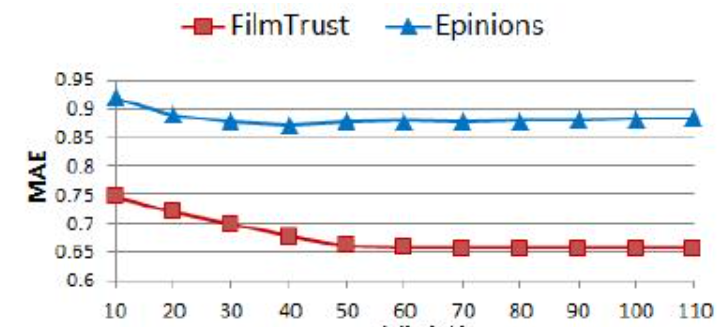
\includegraphics[width=0.4\textwidth]{figures/parameter1.png} %插入图片,[]中设置图片大小,{}中是图片文件名
    \caption{Effect of interation on MAE} %最终文档中希望显示的图片标题
    \label{Fig.2: Effect of interation on MAE} %用于文内引用的标签
    \end{figure}
 \\

    \begin{figure}[H] %H为当前位置,!htb为忽略美学标准,htbp为浮动图形
        \centering %图片居中
        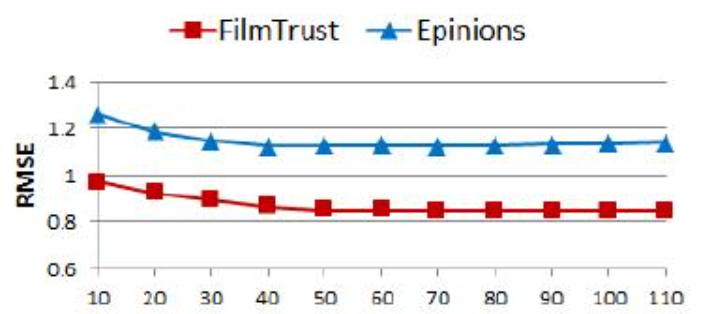
\includegraphics[width=0.4\textwidth]{figures/parameter2.png} %插入图片,[]中设置图片大小,{}中是图片文件名
        \caption{Effect of interation on RMSE} %最终文档中希望显示的图片标题
        \label{Fig.2: Effect of interation on RMSE} %用于文内引用的标签
        \end{figure}
\\
In addition to the number of iterations, the dependence of the predicted ratings on 
the user's own preferences, the weight of localized trust in the trustworthiness, and 
the common rating threshold of two users, etc., all have an impact on the recommendation 
results of trust algorithms\cite{b26}. Due to the limitation of space, we will not go further 
in this Seminar.